\documentclass[12pt]{extarticle}
\usepackage{tikz}
\usetikzlibrary{calc}
\usepackage{eso-pic}
\usepackage{datetime}
\usepackage{lipsum}
\usepackage{graphicx}
\graphicspath{ {/home/pratik/Desktop/}}
\AddToShipoutPictureBG{%
\begin{tikzpicture}[overlay,remember picture]
\draw[line width=6pt]
    ($ (current page.north west) + (0.8cm,-0.8cm) $)
    rectangle
    ($ (current page.south east) + (-0.8cm,0.8cm) $);
\draw[line width=1.5pt]
    ($ (current page.north west) + (1.2cm,-1.2cm) $)
    rectangle
    ($ (current page.south east) + (-1.2cm,1.2cm) $);
\end{tikzpicture}
}
\usepackage{listings}
\usepackage{color}
\date{}
\author{\textbf{Vaibhav Vashisht} 2016CSJ0002  \\\textbf{Pratik Parmar} 2016CSJ0049}
\title{\textbf{CSL216: Computer Architecture\\ Design Document \\ ARM Assembly Simulator  }}
\begin{document}
\maketitle
\newpage
\tableofcontents
\newpage
\section{Introduction}

\subsection{Purpose}
The purpose of this document is to describe the implementation of ARM Assembly Program Simulator application developed by us.
\subsection{Scope}
The software acts as a Assembler for ARM Assembly Code. It runs the ARM assembly code and display the resister's value at any desired instruction in the Assembly code. It also give statistics about the instruction count, CPI, IPI etc at the end of the output. Due to incorparation of pipelining in the simulator,it produces the output in minimum number of cycles possible(At which giving correct ans is feasible) for the assembly code. 
\subsection{Definitions}
\begin{enumerate}
\item \textbf{Pipelining:} Pipelining is an implementation technique where multiple instructions are overlapped in execution. The computer pipeline is divided in stages. Each stage completes a part of an instruction in parallel. The stages are connected one to the next to form a pipe - instructions enter at one end, progress through the stages, and exit at the other end. 
\item \textbf{Hazard:} Hazards are problems with the instruction pipeline in CPU microarchitectures when the next instruction cannot execute in the following clock cycle, and can potentially lead to incorrect computation results. 
\begin{enumerate}
\item \textbf{Data Hazard:} They arise when an instruction depends on the result of a previous instruction in a way that is exposed by the overlapping of instructions in the pipeline.
\item \textbf{Control Hazard:} They arise from the pipelining of branches and other instructions that change the PC.
\item \textbf{Structural Hazard:} They arise from resource conflicts when the hardware cannot support all possible combinations of instructions in simultaneous overlapped execution.
\end{enumerate}
\item \textbf{Forwarding:} Operand forwarding (or data forwarding) is an optimization in pipelined CPUs to limit performance deficits which occur due to pipeline stalls. 
\item \textbf{Stall:} A bubble or pipeline stall is a delay in execution of an instruction in an instruction pipeline in order to resolve a hazard. 
\end{enumerate}
\section{Overall Design}
In this Simulator input file("input.txt") which contains the ARM assembly code will be given. The Simulator will interpretes the input and also generator any error occuring in the code (We have implemented Panic Mode error recovery).
\subsection{Components of Simulator}
\begin{enumerate}
\item \textbf{Instruction Class:}
The class \textbf{Instruction} consists store information about each Instruction:
\begin{enumerate}
\item \textbf{Type}
\item \textbf{Destination Register: }
\item \textbf{Register Operand1:} Returns the index of the component i.e if resistor name is r1 then it returns 1.
\item \textbf{Register Operand}
\item \textbf{Offset:} Offset information for LDR command.
\end{enumerate} 
\item \textbf{Pipeline Class:}
This class consists of Register values information.
\begin{enumerate}
\item It contains all the information related to the instruction in it.
\end{enumerate}

\end{enumerate}
\section{Algorithm}
We will divide each instruction into five stages as done in pipeline.
\begin{enumerate}
\item IF(Instruction Fetch)
\item ID(Instruction Decode)
\item EX(Execute)
\item MEM(Memory)
\item WB(Write Back)
\end{enumerate}
We will make generalized portion in a functions which will handle every type of instruction lets call them stage1,stage2,stage3,stage4,stage5.\\
stage1 will handle IF for every instruction,similarly stage2 will handle ID for each type of instruction and so on.\\
We have improved our parsing and have made the data of each instruction available as data portion of a class.\\
For eg if we want to extract instruction type we can easily extract it from {Instruction Object}.Type() function.These functions are used for making stage1,stage2 etc. Making f1,f2 etc portion is trivial as we just have to replicate the datapath of the final circuit which we made in processor chapter as given below.\\
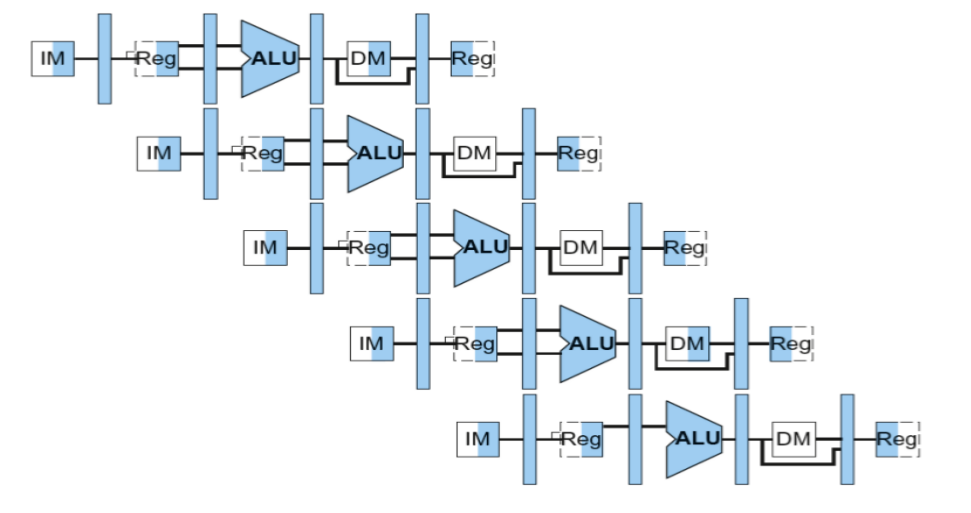
\includegraphics[height=8cm, width=14cm]{PC.png}
\\
Let's explain how will these functions work for instruction add.
stage1 will extract the complete instruction from the class and pass on to IF/ID pipeline.In the next clock cycle stage2 will start decoding the instruction and will extract register number,instruction type(these will be extracted from object of class) and also read register if required and pass onto the next pipeline register.
stage3 will add numbers if command being considered is add,stage4 will store the correspoding values in memory(array here) and stage5 will write back to register.The above mentioned text is very trivial and seems to be very similar to what we studied in processor chapter but differnece will be illustarated through code.
\\
Now comes the part of how to organise these functions so that we can get a pipeline.For this we will take help of recursion.Let's explain this - :
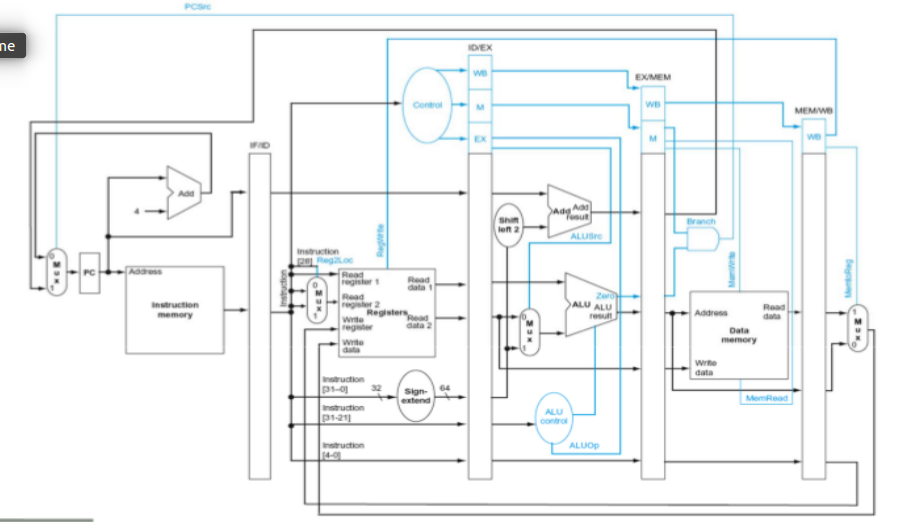
\includegraphics[height=8cm, width=14cm]{PC2.png}
\\
This image above illustrates how pipeline works.
The above function completely illustrates our algorithm for implementing pipeline. They illustrate that ID function for ith instruction after its compeletion will call IF for the next instruction,this will ensure that we get the work done within a clock cycle.
\\
For pipeline also we will have a class which will have pipeline registers as their data component.Also control values will also be contained in the pipeline.
\\
Now lets move to handling hazards.\\
\paragraph{Data Hazard}
We will compare registers for EX/MEM stage and ID/EX stage if we find destination register of EX/MEM stage to be used in ID/EX stage then we know its a data hazard.This can done in f3 function which simulates execute stage using an if condition for comparing two pipeline registers.Now this hazard needs to be removed.\\
													This is done by extracting the needed value from the 
EX/MEM pipeline register.This is incorporated by putting an if statement in the execute state function which checks if the given conditon holds then value is extracted from the pipeline register of the next stage .
\lstinputlisting[language=Java]{Test2.s}
\paragraph{Load-Use Hazard}
Similar to data hazard these are detected by comparing ID/EX and IF/ID pipeline registers.This is resolved by inserting a stall into the pipeline.How do we insert a stall ?\\
We maintain a bool variable which be passed onto all the stages of the pipeline and that varaible if true will not allow any data to be written into the regsiters and memory.\\
Alternatively we can also implement as done in arm pipeline.We will turn all control values to zero and hence nothing will be allowed to written to registers or memory.This can be done in the f2 function which then propagates to the next stages of the pipeline.\\
															We also have to stop increment of pc until we have stalls, this can be done by decrementing pc in f2 which will again get incremented by default and hence will fetch the same instruction.\\
Different number of clock cycles for some instructions -:\\
This means that some stages of these instrcution will take more than one clock cycle hence we need to stall till that stage gets completed.Stalling is done as described in the load use hazard by setting control values to zero.
\lstinputlisting[language=Java]{Test3.s}

\paragraph{Branch Hazard}
 One simple way is to stall the pipeline till we are not sure where will branch move pc to.As we have implemented branch instructions based on cmp statement placed above the branch statement hence we have to stall after cmp for it to be able to compare the values till execute stage.After that we can directly direct that value(true or false) to the first stage of branch and there on branch or not.But to make pipeline more aggressive we need to use branch prediction for which we may have to flush all the stages of pipeline extracted due to taking wrong prediction.This can be done by maintaining a global variable which can be turned true when we detect that we have taken the wrong branch(This can be detected upto EX or MEM stage),hence we need to flush atmost 4 pipeline stages.After the global variable is turned true we can simply zero all the wrongly taken stages by making all signals and values in them to be zero as a result no wrong values propagate in next stages.Also we need to change pc,this can also be done by an if condition on global variable which will hence change pc.
 \lstinputlisting[language=Java]{Test6.s}    
\paragraph{Structural Hazard}
This are automatically removed by maintaining different arrays for storage.
\paragraph{Assumptions}
For each round in the pipeline, each stage in the pipeline will take maximum of cycles required by any pipeline.
\paragraph{•}
Sequence of Execution in function Operate():\\
\begin{center}
Write Back(Stage 5) \\ Memory (Stage 4) \\ Execute (Stage 3) \\ Instruction Decode (Stage 2) \\ Instruction Fetch (Stage 1)\\
\end{center}
For passing a NOP instruction, we pass 9999 into the function.(This works as a code for NOP instruction).\\
In the starting each pipeline register will be in nop state therefore no operation will be performed in stage 5 to stage 2, then only in stage 1 Instruction fetch will happen.\\
Then continuously instruction will be passed in the function and earlier instruction in the operate function will go up in stage and finally leave when write back stage would happen for them.\\
Similarly at the end 4 extra NOP instructions are passed in the pipeline to get last instruction to complete it's write back. 
\subsection{Instruction Handling}
\begin{enumerate}
\item \textbf{ADD,SUB(etc arithmetic operations)}\\ 
Decoding and fetching stages will be common to all type of instructions but EX stage will be dfiferent for arithmetic operations in this stage these instructions will use ALU to calculate the result and send to the next stage pipeline registers.
\item \textbf{STORE,LOAD(memory type operations)}\\ 
In these type of operations memory stage will be active and other stage will be similar to the rest of the instructions but in memory stage these instructions will either read or write from the memory.These instructions may also require execute stage when load,str with offset are used.
\item \textbf{B,BL,BNE(etc)}\\ 
In this in the first stage and second stage as in all instructions just fetch decode happens,nothing happens in IF and Execute stage of this instruction when BNE reaches MEM stage CMP would have reached the final stage and we would have already got the result of comparison in the execute stage hence we would accordingly flush the instructions/continue with inserted instructions in the pipeline.
\item \textbf{For 'B'}\\ 
Firstly instruction is fetched and when 'B' instruction is decoded directly the instrcution after the label is fetched.  
\item \textbf{For 'BL'}\\ 
It is just similar to B instruction just that link register value is updated with pc+1.
\item \textbf{For CMP}\\ 
In this first and second stage happen normally and in the third stage comparator is used to compare the two values when we reach the fourth stage in the comparator new instructions are fetched according to the result. 
\end{enumerate}
\section{Testing}
\subsection{TestCases}
\begin{enumerate}
\item \lstinputlisting[language=Java]{Test1.s}
Testcase with load-use and data hazard.
\item \lstinputlisting[language=Java]{Test2.s}
Testcase with Data hazard.
\item \lstinputlisting[language=Java]{Test3.s}
Testcase with load-use and data hazard.
\item \lstinputlisting[language=Java]{Test4.s}
Testcase with data and control hazard.
\item \lstinputlisting[language=Java]{Test5.s}
Testcase with load-use hazard.
\item \lstinputlisting[language=Java]{Test6.s}
Testcase with data and control hazard.
\item \lstinputlisting[language=Java]{Test7.s}
Testcase with control and data hazard along with the use of link register.
\item \lstinputlisting[language=Java]{Array.s}
Testcase for iteration in an array using branch.
\item \lstinputlisting[language=Java]{Fibonacci.s}
Testcase for finding fibonacci at a given position.
\end{enumerate}

\section{Software Requirement}
Following Software/Packages are Required for running this application.
\begin{enumerate}
\item GNU g++ Compiler for C++ 11\\
For Compilation of C++ program
\end{enumerate}


\end{document}